% generated by scripts/pkl_to_latex.py
% source PKL : uscan_v1_L8_Ne8_t1_mode-uniform_nmin2_solver-gcg_full_es_restarts8_iter200_kmax4_tol1em09_U0.1to5_N20-0abb1d3c527c.pkl
% scan type  : uscan
% state      : ex_singlet
% requires   : \usepackage{pgfplots} \pgfplotsset{compat=1.18}
% colours match the matplotlib PDF (tab10 cycle)
\definecolor{gmeC0}{HTML}{1F77B4}
\definecolor{gmeC1}{HTML}{FF7F0E}
\definecolor{gmeC2}{HTML}{2CA02C}
\definecolor{gmeC3}{HTML}{D62728}
\definecolor{gmeC4}{HTML}{9467BD}
\definecolor{gmeC5}{HTML}{8C564B}
\definecolor{gmeC6}{HTML}{E377C2}
\definecolor{gmeC7}{HTML}{17BECF}

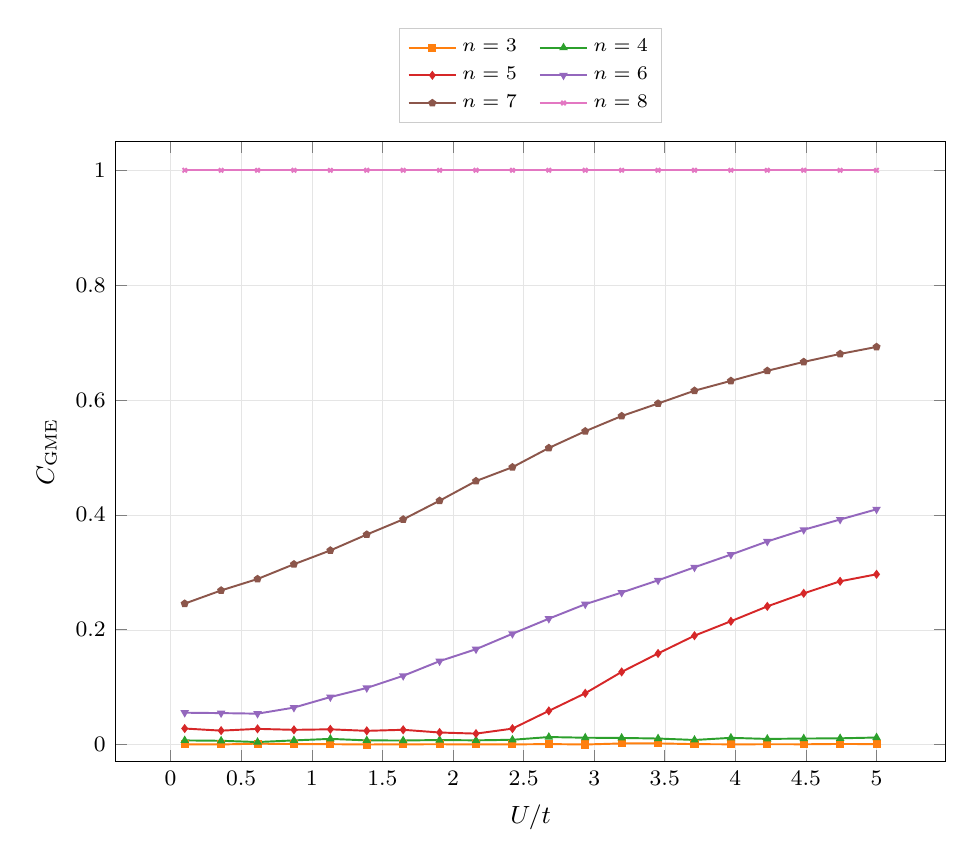
\begin{tikzpicture}
  \begin{axis}[
    width=\columnwidth,
    height=0.78\columnwidth,
    xlabel={$U/t$},
    ylabel={$C_{\mathrm{GME}}$},
    grid=both,
    grid style={line width=.1pt, draw=gray!20},
    tick label style={font=\footnotesize\rmfamily, /pgf/number format/fixed},
    label style={font=\small\rmfamily},
    scaled ticks=false,
    legend style={font=\scriptsize\rmfamily, draw=gray!40, at={(0.5,1.03)}, anchor=south, /tikz/every even column/.append style={column sep=6pt}},
    legend cell align={left},
    legend columns=2,
    ymin=-0.03,
    ymax=1.05,
  ]
    \addplot[color=gmeC1, mark=square*, mark size=1.1pt, line width=0.7pt] coordinates {
        (0.1,0.000114) (0.357895,0.000087) (0.615789,0.001479) (0.873684,0.000771)
        (1.131579,0.000587) (1.389474,0.000015) (1.647368,0.000331) (1.905263,0.000465)
        (2.163158,0.000136) (2.421053,0.000171) (2.678947,0.000767) (2.936842,0.000046)
        (3.194737,0.001848) (3.452632,0.001941) (3.710526,0.000667) (3.968421,0.000318)
        (4.226316,0.000449) (4.484211,0.00039) (4.742105,0.000983) (5,0.000684)
    };
    \addlegendentry{$n=3$}
    \addplot[color=gmeC2, mark=triangle*, mark size=1.1pt, line width=0.7pt] coordinates {
        (0.1,0.007128) (0.357895,0.006503) (0.615789,0.004304) (0.873684,0.007142)
        (1.131579,0.009814) (1.389474,0.007152) (1.647368,0.006968) (1.905263,0.007834)
        (2.163158,0.007239) (2.421053,0.008248) (2.678947,0.013013) (2.936842,0.011836)
        (3.194737,0.011445) (3.452632,0.010416) (3.710526,0.007915) (3.968421,0.011618)
        (4.226316,0.009728) (4.484211,0.010392) (4.742105,0.010795) (5,0.012183)
    };
    \addlegendentry{$n=4$}
    \addplot[color=gmeC3, mark=diamond*, mark size=1.1pt, line width=0.7pt] coordinates {
        (0.1,0.027849) (0.357895,0.024143) (0.615789,0.027246) (0.873684,0.025562)
        (1.131579,0.026478) (1.389474,0.023795) (1.647368,0.025644) (1.905263,0.020902)
        (2.163158,0.018975) (2.421053,0.027663) (2.678947,0.058567) (2.936842,0.089223)
        (3.194737,0.126424) (3.452632,0.158594) (3.710526,0.189535) (3.968421,0.214698)
        (4.226316,0.24052) (4.484211,0.263231) (4.742105,0.284228) (5,0.296422)
    };
    \addlegendentry{$n=5$}
    \addplot[color=gmeC4, mark=triangle*, mark size=1.1pt, mark options={rotate=180}, line width=0.7pt] coordinates {
        (0.1,0.055378) (0.357895,0.054705) (0.615789,0.053719) (0.873684,0.064317)
        (1.131579,0.08264) (1.389474,0.098469) (1.647368,0.119611) (1.905263,0.145166)
        (2.163158,0.165978) (2.421053,0.192812) (2.678947,0.219116) (2.936842,0.244316)
        (3.194737,0.264657) (3.452632,0.285941) (3.710526,0.308621) (3.968421,0.33069)
        (4.226316,0.353642) (4.484211,0.373937) (4.742105,0.391821) (5,0.409605)
    };
    \addlegendentry{$n=6$}
    \addplot[color=gmeC5, mark=pentagon*, mark size=1.1pt, line width=0.7pt] coordinates {
        (0.1,0.245384) (0.357895,0.268317) (0.615789,0.288214) (0.873684,0.313936)
        (1.131579,0.337994) (1.389474,0.365647) (1.647368,0.392039) (1.905263,0.42457)
        (2.163158,0.458815) (2.421053,0.482881) (2.678947,0.516415) (2.936842,0.545576)
        (3.194737,0.572022) (3.452632,0.59383) (3.710526,0.616146) (3.968421,0.633282)
        (4.226316,0.650769) (4.484211,0.66628) (4.742105,0.680208) (5,0.692366)
    };
    \addlegendentry{$n=7$}
    \addplot[color=gmeC6, mark=x, mark size=1.1pt, line width=0.7pt] coordinates {
        (0.1,1) (0.357895,1) (0.615789,1) (0.873684,1)
        (1.131579,1) (1.389474,1) (1.647368,1) (1.905263,1)
        (2.163158,1) (2.421053,1) (2.678947,1) (2.936842,1)
        (3.194737,1) (3.452632,1) (3.710526,1) (3.968421,1)
        (4.226316,1) (4.484211,1) (4.742105,1) (5,1)
    };
    \addlegendentry{$n=8$}
  \end{axis}
\end{tikzpicture}
